\documentclass{article}
\usepackage[utf8]{inputenc}
\usepackage{graphicx}
\usepackage{fancyhdr}
\usepackage{geometry}
\usepackage{amsmath}
\usepackage{amssymb}
\usepackage{url}
\usepackage{hyperref}

\geometry{left = 2.5cm, right=2.5cm, bottom=2.5cm, top=2.5cm}

\title{3806ICT - Week 3 Lab}
\author{Nick van der Merwe - s5151332 - nick.vandermerwe@griffithuni.edu.au}

\pagestyle{fancy}
\renewcommand{\headrulewidth}{1pt}
\fancyhf{}
\rhead{3806ICT - Exercises w1-5}
\chead{Griffith University}
\lhead{Nick van der Merwe - s5151332}
\rfoot{Page \thepage}
\newcommand\tab[1][1cm]{\hspace*{#1}}

\begin{document}
\maketitle

%==============================================================================
\section*{Question 1}
\textbf{\textit{
    \tab Give  definitions  of  locomotion  and  manipulation.  What  are  their shared features and differences?  
}} \\ \\
Locomotion is defined as a robot's ability to move itself by exerting force on 
the environment whereas manipulation is its ability to move objects by 
exerting force upon them.
%==============================================================================
\section*{Question 2}
\textbf{\textit{
    \tab What are advantages and disadvantages of legged robots?
}} \\ \\
Easiest format to see this in would be lists:
\subsubsection*{Advantages}
\begin{itemize}
    \item They can go over more complicated obstacles without 
        getting stuck (slanted ground, steps, et cetera)
    \item Causes less damage to terrain than wheeled robots
\end{itemize}
\subsubsection*{Disadvantages}
\begin{itemize}
    \item Movement speed
    \item Complexity - actuators and structure are a lot more complicated
    \item Harder to control - must consider balance and stability
    \item Less energy efficient due to:
    \begin{itemize}
        \item Terrain
        \item Centre of gravity moves while walking
        \item Picking up the legs
    \end{itemize}
\end{itemize}
%==============================================================================
\section*{Question 3}
\textbf{\textit{
    \tab What is DOF? If a robot can only move forward and backward, 
    how many DOFs does it have? In most cases, how many DOFs does a robot leg has?
}} \\ \\
DOF stands for \textbf{d}egrees \textbf{o}f \textbf{f}reedom, and its defined by the
number of joins in each leg. To have a leg that only moves forwards and backwards,
it would have two joints: this is because its limited to doing a lift and swing motion.
To move backwards it just swings in the other direction than normal. Most robot legs
have three joints.
%==============================================================================
\newpage
\section*{Question 4}
\textbf{\textit{
    \tab What is a gait of a legged robot? Enumerate all lift and release 
    events of a robot with 4 legs. Give two examples of gaits for such a robot.
}} \\ \\
Our formula to find how many states there are is $2^k = 2^4 = 16$ states.
\begin{figure}[ht]
    \centering
    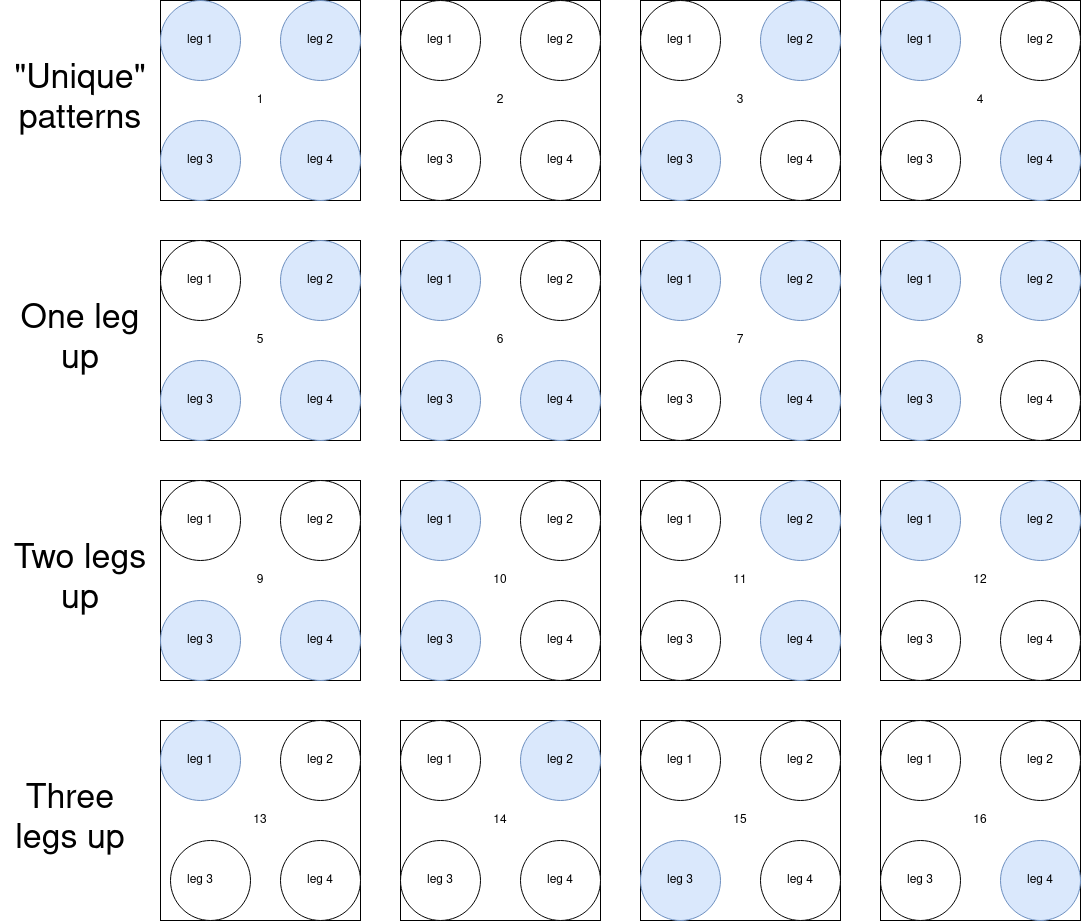
\includegraphics[width=0.5\textwidth]{img/gait.png}
    \caption{Blue means a leg is down and white is the leg is up}
\end{figure}

Now to depict two gaits of a four legged robot:
\begin{figure}[ht]
    \centering
    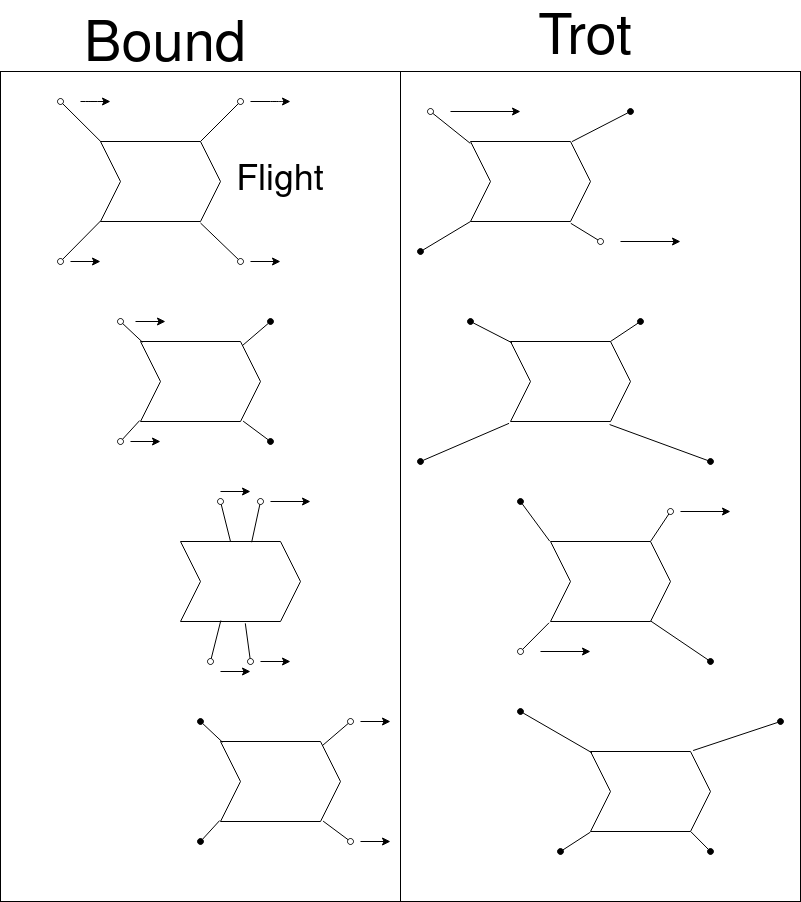
\includegraphics[width=0.4\textwidth]{img/gait-walk.png}
\end{figure}
\newpage
%==============================================================================
\section*{Question 5}
\textbf{\textit{
    \tab Formulate the Monkey and Banana Problem in STRIPS:A monkey is at location A in a lab. There is a box in location C. The monkey wants the bananas that are hanging from the ceiling in location B, but it needs to move the box and climb onto it in order to reach them
}} \\ \\
%//////////////////////////
\textbf{States}
\begin{itemize}
    \item \underline{Initial State} MonkeyLocation(A), MonkeyLevel(low), BoxLocation(C), BananasLocation(B),
    \item \underline{Goal state} Have(bananas)
\end{itemize}

\subsection*{Actions}
\begin{itemize}
    \item \_Move(X, Y)\_
        \begin{itemize}
            \item Pre: Box(X), Location(?Y) HandsFree(), MonkeyNOTOnBox(?X), 
                MonkeyLocation(?Y), At(X, Y)
            \item Effects+: Carrying(?X), 
            \item Effects-: FreeHands(), At(?X, ?Y)
        \end{itemize}
    \item \_MoveBox(FromPlace, ToPlace)\_
        \begin{itemize}
            \item MonkeyLocation(FromPlace), BoxLocation(FromPlace), MonkeyLevel(low)
            \item BoxLocation(ToPlace), not BoxLocation(FromPlace), MonkeyLocation(ToPlace), not MonkeyLocation(FromPlace)
        \end{itemize}
    \item \_ClimbUp(Place)\_
        \begin{itemize}
            \item AtLocation(Place), BoxAt(Place), MonkeyLevel(low)
            \item MonkeyLevel(high), not MonkeyLevel(low)
        \end{itemize}
    \item \_TakeBananas(Place)\_
        \begin{itemize}
            \item MonkeyLocation(Place), BananasLocation(Place), MonkeyLevel(high)
            \item Have(Bananas)
        \end{itemize}
\end{itemize}
%==============================================================================
\section*{Question 6}
\textbf{\textit{
    \tab Evaluate  the  subsumption  architecture  in  terms  of:  support  for modularity, niche targetability, 
    ease of portability to other domains, robustness
}} \\ \\
% Modularity: Does it show good software engineering principles?
There are two perspectives on whether subsumption has good modularity.
Firstly, its granted hea  subsumption is a form of the reactive 
paradigm and its main architecture revolves around modules, 
it can be considered as highly modular. This is especially visible as 
modules are layered and reflects parts of object oriented programming as 
they have the ability to override, 
subsume and contain one another (when they're layered). 
Only thing that's arguably missing is inheritance, but 
that can probably be simulated by layering as well. \\
\tab The counter argument to this is that its very rarely
taken advantage of in practice when subsumption is used \cite{FangTang}. 
Overall, one would say there's more argument that its modularity is high as
it's capable of many OOP properties - even if it's rarely used.
\\
% Niche Targetability: How well does it work for the intended application? Lecture 5 1:20:18 he mentions this
\tab 
The niche targetability is high as we can design the system in a very specific way depending on the situation.
For instance, it can compile down onto a programmable-array logic circuit \cite{FangTang}.
\\
% Ease of portability to other domains: How well would it work for other applications or other robots? 1:21:55 lecture 5
\tab For portability, due to the fact that the system operates in layers 
if we tried to adjust an existing robot to a different application
chances are that it would take too much effort to do. As in, if 
there's a fundamental behaviour in layer 0, or even
the second last layer that we want to change it could be a lot 
of effort. On top of this, adapting to picking
different actions based on stimulus is challenging
For this reason its portability is quite low, which 
is different from a reactive paradigm. \cite{IntroToAI} \\
% Robustness: Where is the system vulnerable, and how does it try to reduce that vulnerability
\tab Overall its robustness to failure is arguable. 
Sensors failing is usually detected, and can be countered by having 
more than than the minimum number of sensors. 
Furthermore, the lower layers will continue to operate when higher ones
are added, however, the problem arises at high layers. 
These can only inhibit and suppress lower layers as they actively
interfere with them, and therefore they can cause undetected 
errors in the robot. Due to this its robustness is typically
evaluated as low because there is no inbuilt method to identify 
these failures. \cite{IntroToAI} \cite{reactiveParadigms}
\\
\tab In summary, it's modularity is good since it has many OOP functions and the niche targetability is high as it can be programmed
on very low level systems. 
It's main weakness out of the four is its ease of portability to different uses, and its robustness to failure
is generally considered low.

%==============================================================================
\section*{Question 7}
\textbf{\textit{
    \tab Describe the Hybrid paradigm in terms of: (a) sensing, acting, and planning, and (b) sensing organization.
}} \\ \\

Basically the planning is done on its own, and the sensing and acting are done together. That's to say that information,
sensed or cognitive, is put through the plan paradigm and that gives us directives. These directives allow our sense-act
section to decide what to do when it senses information. Its 'hybrid-ness' is visible through this, as it introduces
planning from other architectures into a reactive architecture's sensing and acting.
This assists with the downside of the subsumption model having difficulty adapting different actions 
to senses that are similar. The specific way P, SA acts is visible in figure \ref{HybridPSA}.

\begin{figure}[ht]
    \centering
    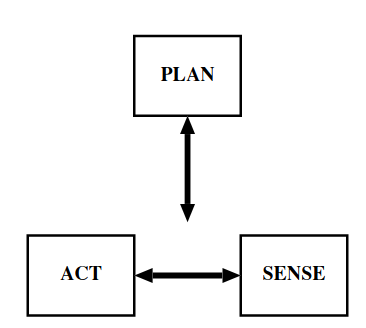
\includegraphics[scale=0.5]{img/PSA-Hybrid.png}
    \caption{The plan, sense act model for hybrid architecture}
    \label{HybridPSA}
\end{figure}

\tab The sensing organisation also merges the hierarchical and reactive styles as both planning and
acting requires the sensory
information. In the model this causes it to be more complex than the hierarchical one, our global world model can have its
own sensor and the behaviours can selectively listen to sensors while being able to create virtual sensors.
An example is visible in figure \ref{sOrg}.
\begin{figure}[ht]
    \centering
    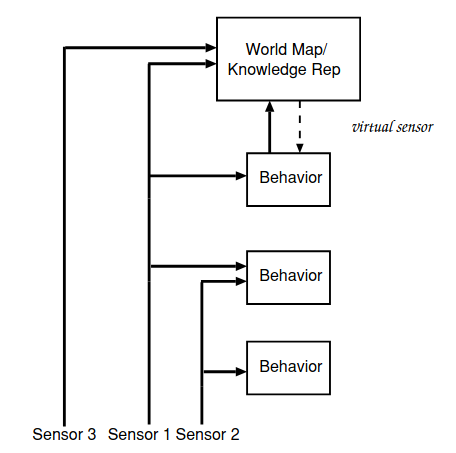
\includegraphics[scale=0.5]{img/sensing-organisation.png}
    \caption{Sensing organisation of hybrid paradigm. Taken from \cite{IntroToAI}}
    \label{sOrg}
\end{figure}
%==============================================================================
\newpage
\section*{Question 8}
\textbf{\textit{
    \tab Look up technical reports on Shakey. Compare Shakey with the Hybrid
architectures.  Now  consider  the  possible  impact  of the  radical  increases  in
 processing power since the 1960’s. Do you agree or disagree with the statement that
Shakey would be as capable as any Hybrid if it were built today? Justify your answer.
}} \\ \\
The overwhelming issue with shakey in terms of its architecture is the fact that
it effectively closed its eyes when it was not in
the sensing stage of its plan-sensing-acting paradigm, which would happen to be majority of the time \cite{IntroToAI}. This is due 
to both the hardware on board (SDS 940 computer \cite{shakey}) and that the STRIPS paradigm is slow. For reference, a SDS 940 computer
has a whopping maximum main of 64 kilowords and is old enough that its processing speed was 
measured by microseconds to add numbers, not hertz.  \\
\tab To try to convert it, it takes 77 microseconds on the SDS 940 to a 24 bit floating operation. 
In other words it has (1/0.000077 = 12987 FLOPS(24 bit)(floating pointer operations per second)) \cite{SDS940}. 
On the other hand, an AMD Ryzen Threadripper 3990X has a whopping 13,209GFLOPS, or 13209000000000 FLOPS (32bit) \cite{threadripper}.
Note that later on Shakey was updated to a PDP-10 \cite{shakey}, but that's still a similar comparison
that its effectively millions of times slower than today's technology. 
\\
\tab Not to mention, in terms of the planning algorithmic speed, the hybrid paradigm has O(n) algorithms \cite{IntroToAI} 
whereas STRIPS planning varies depending on the situation, but will always be 
PSPACE-complete; that is, it will never exceed $O(n^k)$ in complexity. 
\\
\tab However, even if we manage to keep up with STRIPS's much higher demand for processing, the integral problem with 
it still exists: its single threaded. A hybrid can see a situation, plan it, and while its acting if it goes wrong 
it can replan to react to the situation. On the other hand, STRIPS would finish acting out its plan then realise something
went wrong. For this reason, the STRIPS model would have to be changed to compete with hybrid robots.
\newpage

\bibliographystyle{apalike}
\bibliography{biblio}


\end{document}
